\section{Problem Statement}
\label{sec:problem-statement}

The general problem we wish to solve is the variable coefficient elliptic \gls{pde} that we define as
\begin{align}
    \label{eq:elliptic-pde}
    \mathcal{A}[u(\textbf{x})] \equiv \nabla \cdot \left( \beta(\textbf{x}) \nabla u(\textbf{x}) \right) + \lambda(\textbf{x}) u(\textbf{x}) &= f(\textbf{x}), \quad \textbf{x} \in \Omega \subset \mathcal{R}^2
\end{align}
subject to either Dirichlet boundary conditions
\begin{align}
    \label{eq:elliptic-pde-bc1}
    u(\textbf{x}) &= g(\textbf{x}), \quad \textbf{x} \in \Gamma_D \subset \Omega
\end{align}
or Neumann boundary conditions
\begin{align}
    \label{eq:elliptic-pde-bc2}
    \frac{\partial u}{\partial n} \Big|_{\textbf{x}} &= v(\textbf{x}), \quad \textbf{x} \in \Gamma_N \subset \Omega.
\end{align}

\begin{figure}
    \centering
    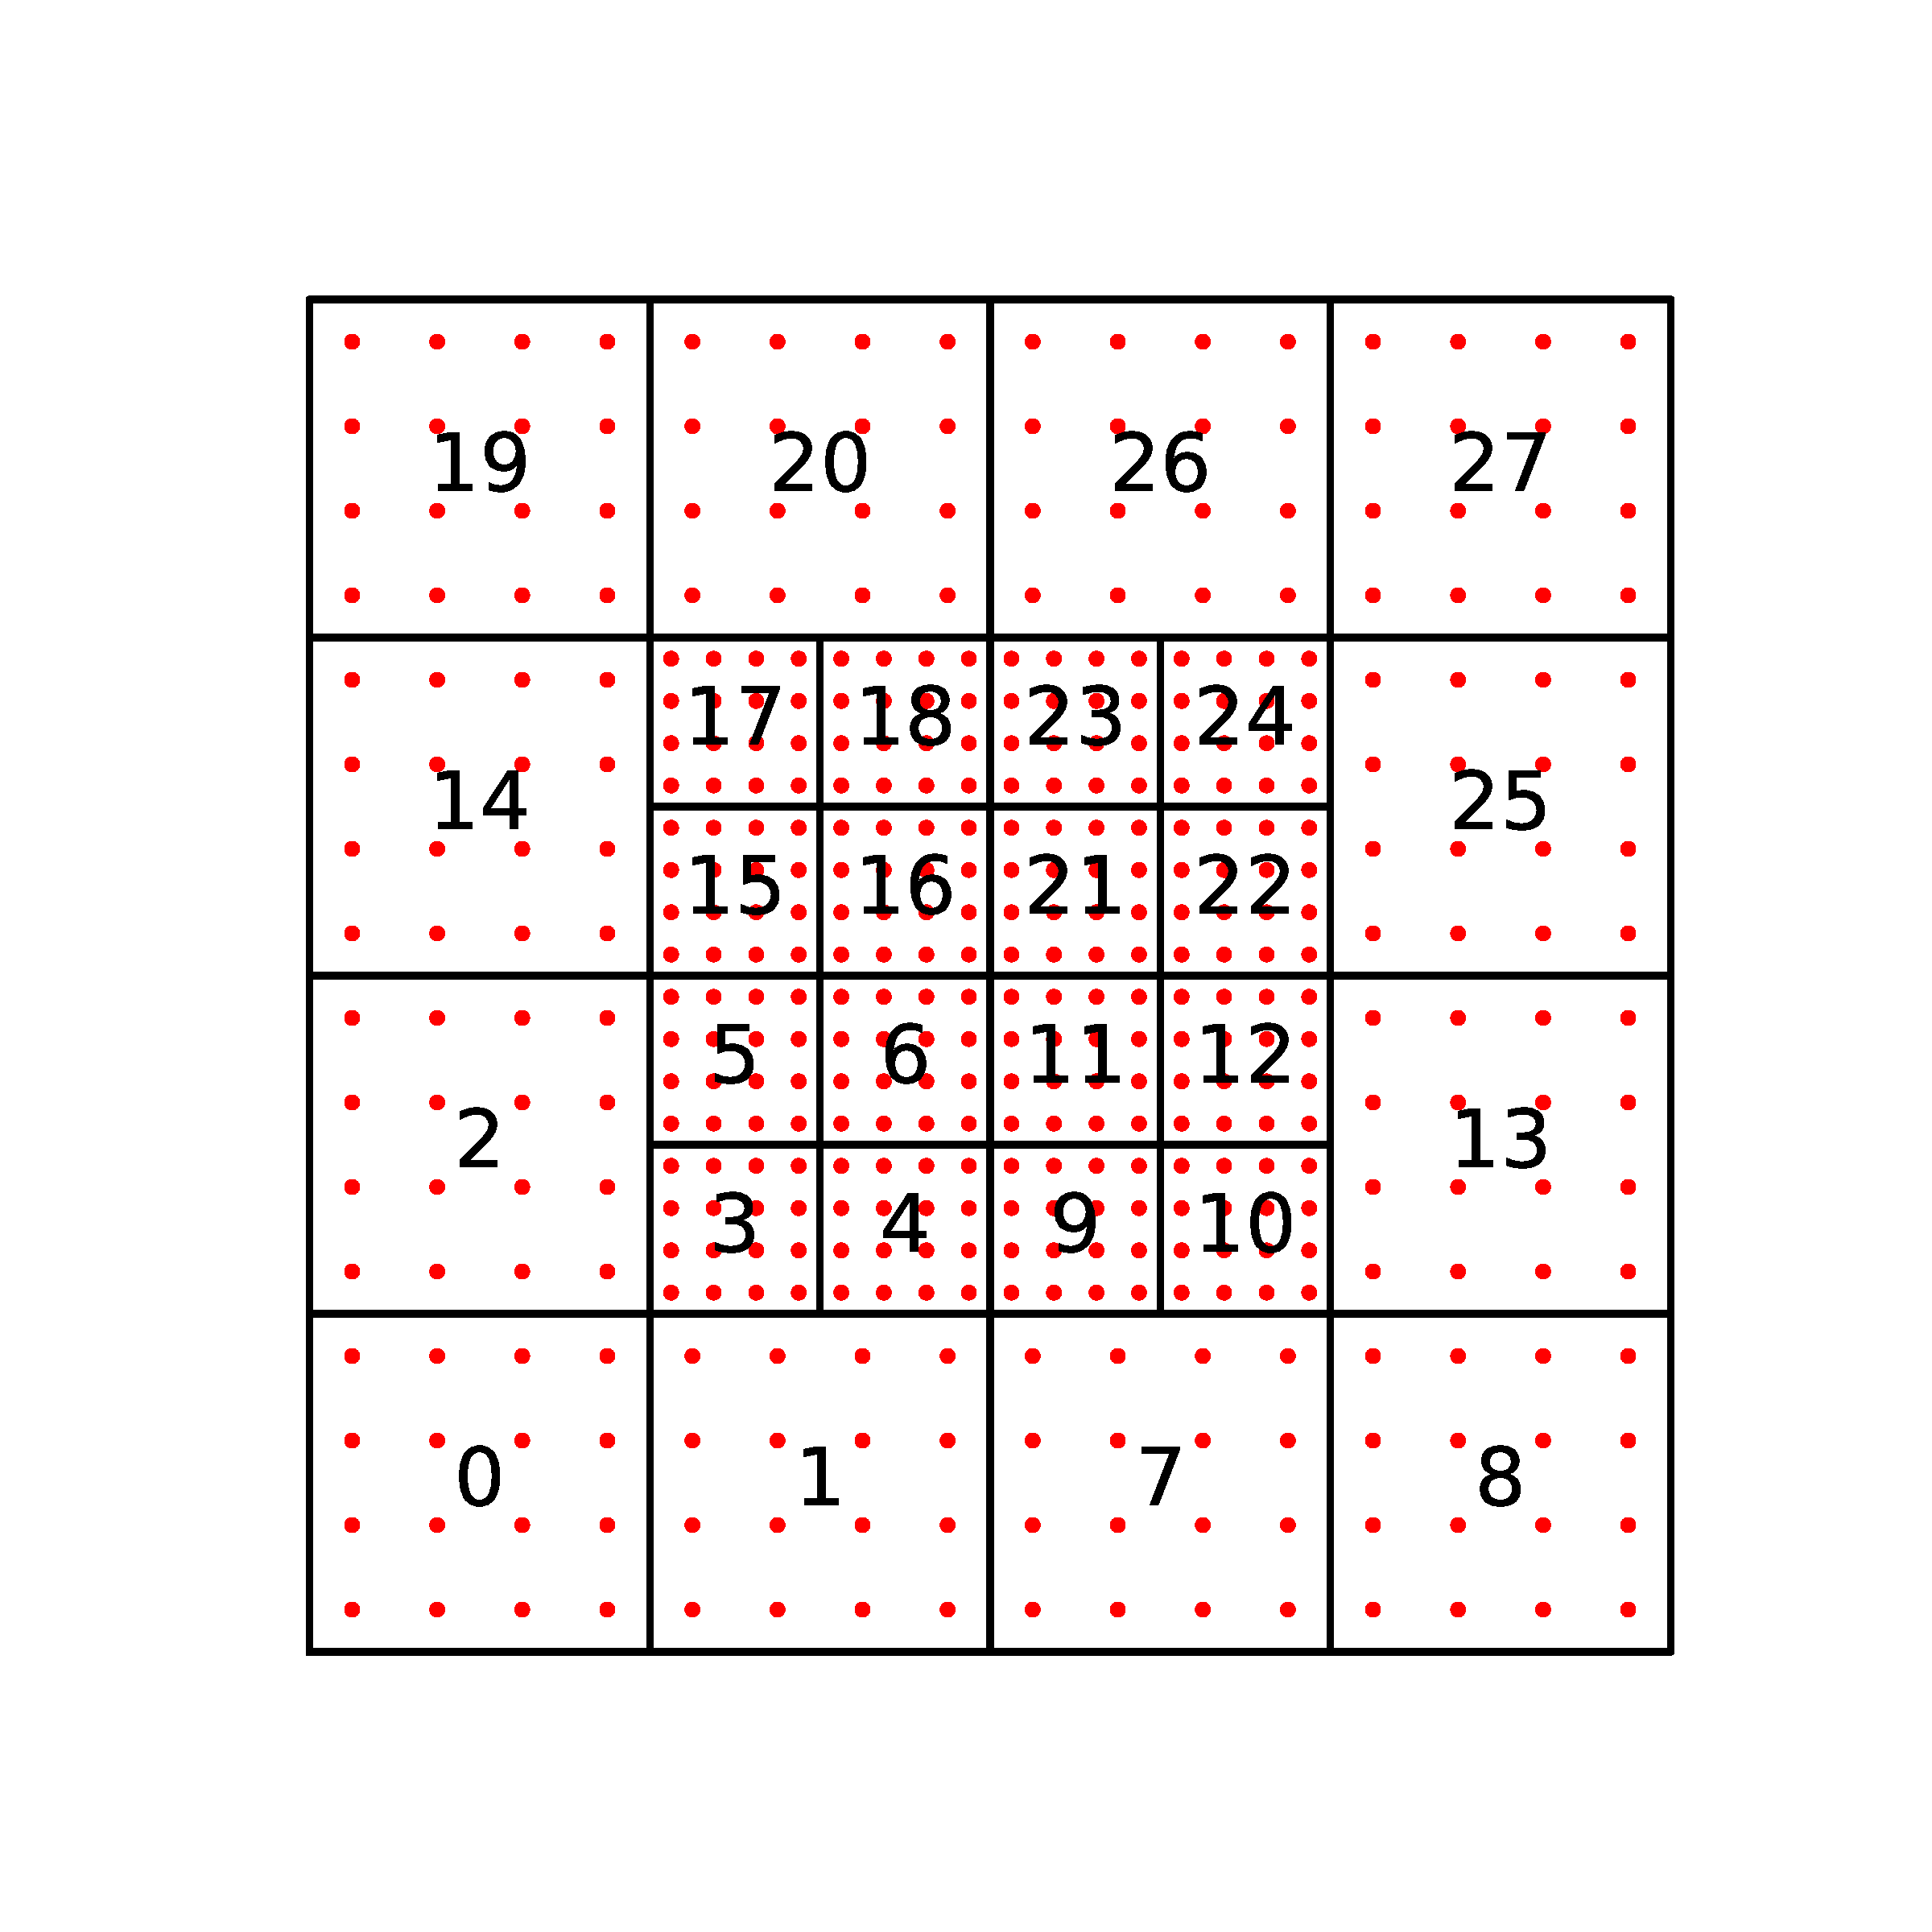
\includegraphics[width=\textwidth, clip=true, trim={0 160 0 160}]{figures/adaptive-mesh-serial.pdf}
    \caption{An example of a domain $\Omega$ refined according to a refinement criteria that refines around the center of the domain. The indices indicate the leaf-level index as organized into a leaf-level quadtree $\mathcal{Q}_L$. Each subdomain has a finite volume discretization associated with it as depicted with the red points.}
    \label{fig:adaptive-mesh-serial}
\end{figure}

The domain $\Omega$ is partitioned into a composite collection of subdomains $\Omega_i$ such that $\Omega = \cup_{i = 1}^{N} \Omega_i$. This is displayed in \reffig{fig:adaptive-mesh-serial}. These subdomains are organized into a {\em leaf-indexed quadtree}
\begin{align}
    \mathcal{Q}_L = \{\Omega_i | i = 1, \dots, N_L\},
    \label{eq:leaf-indexed-quadtree}
\end{align}
where $N_L$ is the number of leaf nodes. \ignore{A representation of the mesh in \reffig{fig:adaptive_mesh} as a leaf-indexed quadtree can be found in \reffig{subfig:leaf-indexed-quadtree}.} Building up $\mathcal{Q}_L$ is done by recursively refining a logically square domain into children patches according to a refinement criteria (or tagging criteria)
\begin{align}
    T_{R} (\textbf{x}) =
    \begin{cases}
        1,& \eta(\textbf{x}) > \epsilon_{R} \\
        0,& \text{otherwise}
    \end{cases}
    \quad \textbf{x} \in \Omega_i,
\end{align}
where $\eta(\textbf{x})$ is a metric used to measure the need for refinement such as error or state variable gradient. A value of $1$ indicates refinement and a value of $0$ indicates no refinement. The user-defined variable $\epsilon_{R}$ is the refinement threshold. While a coarsening criteria $T_{C}$ is also defined similar to the refinement criteria, it is often not used in the initialization of $\mathcal{Q}_L$.

We also define a {\em path-indexed quadtree} that is formally denoted as
\begin{align}
    \mathcal{Q}_P = \{\Omega^{\tau} | \tau = 1, \dots, N_P\},
    \label{eq:path-indexed-quadtree}
\end{align}
where $\tau$ is a key that indicates the path of a node in $\mathcal{Q}_P$ and $N_P$ is the number of nodes in $\mathcal{Q}_P$. The primary difference between a leaf-indexed quadtree and a path-indexed quadtree is the indexing of nodes; a leaf-indexed quadtree has data storage for only leaf nodes while a path-indexed quadtree has data storage for all nodes in the quadtree (leaves and ancestors). Both types of trees are depicted in \reffig{fig:quadtree-indexing-serial}.

\begin{figure}
    \centering
    \begin{tabular}{c}
    \smallskip
        \begin{subfigure}[t]{0.8\textwidth}
            \centering
            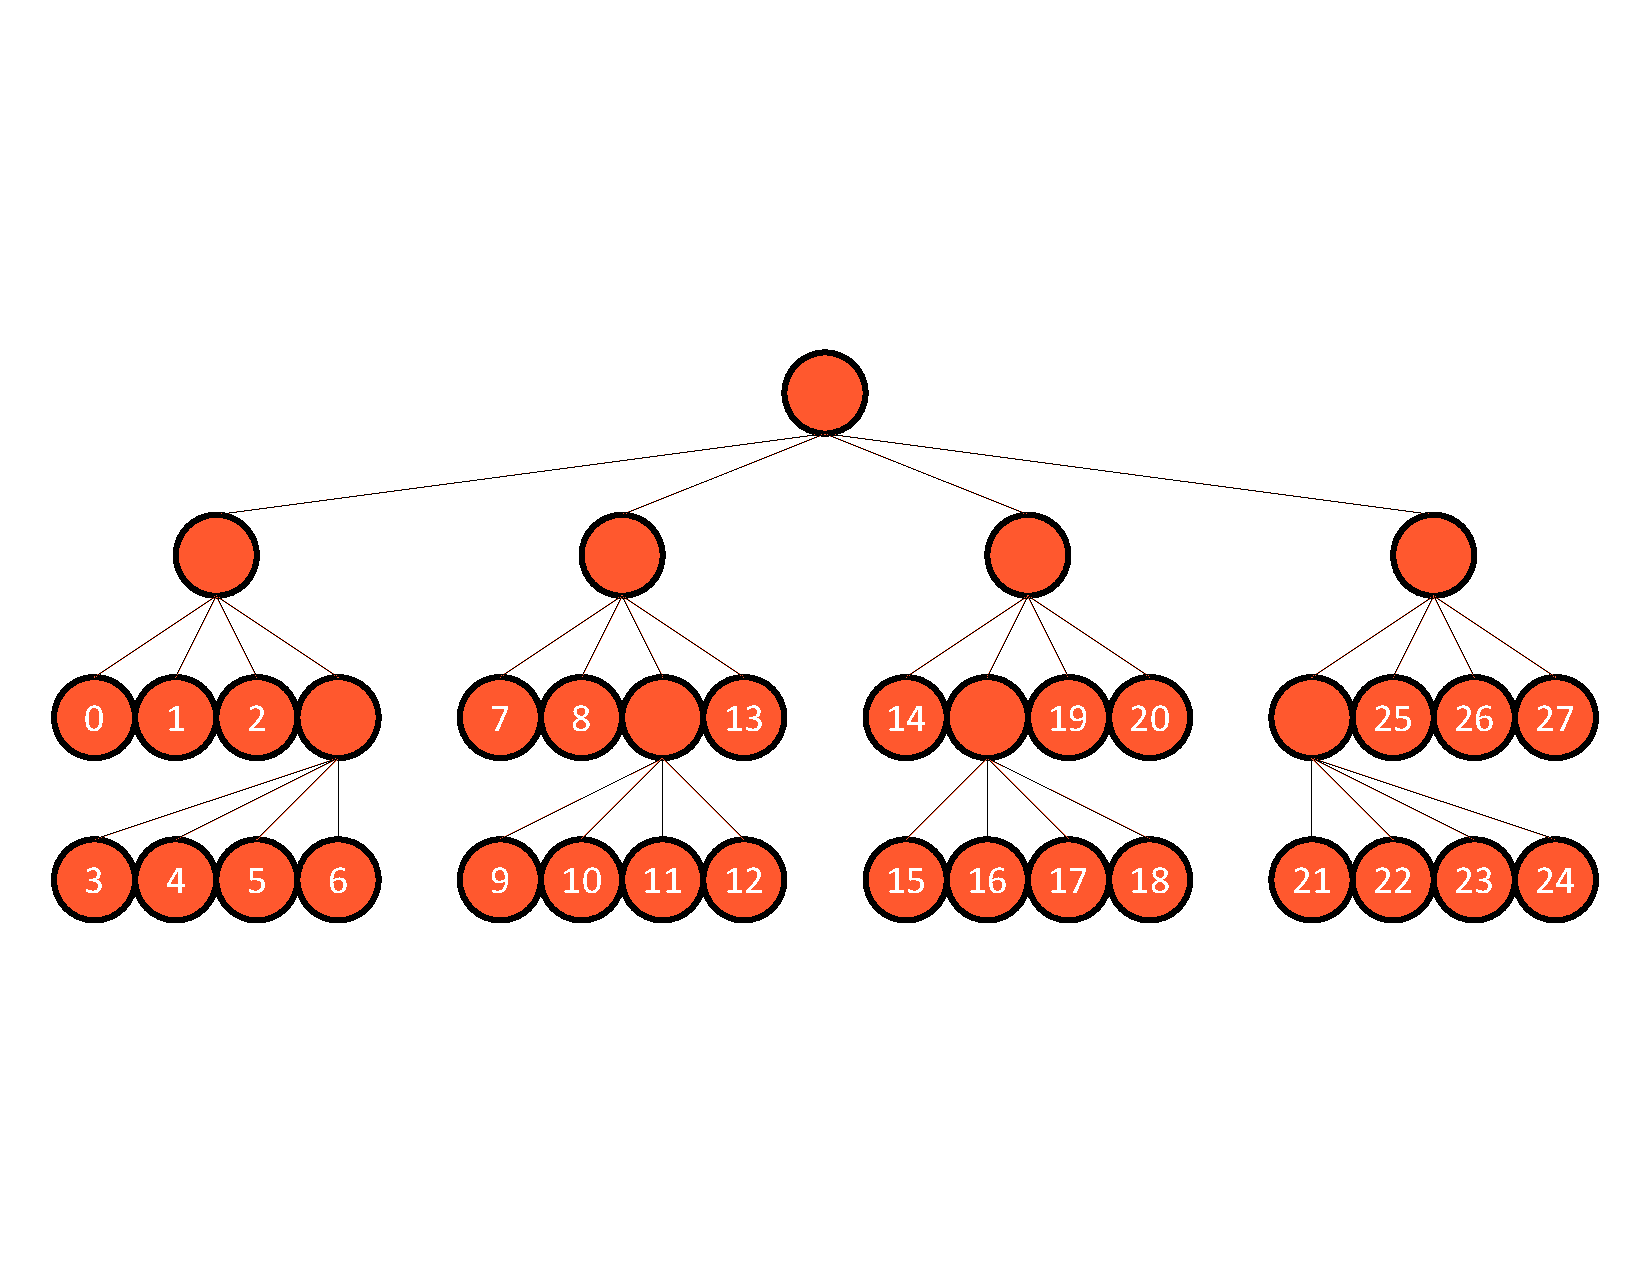
\includegraphics[width=\textwidth, clip=true, trim={0 150 0 150}]{figures/leaf-indexed-quadtree-serial.pdf}
            \caption{Leaf-indexed quadtree $\mathcal{Q}_L$}
            \label{subfig:leaf-indexed-quadtree-serial}
        \end{subfigure}
        \\
        \begin{subfigure}[t]{0.8\textwidth}
            \centering
            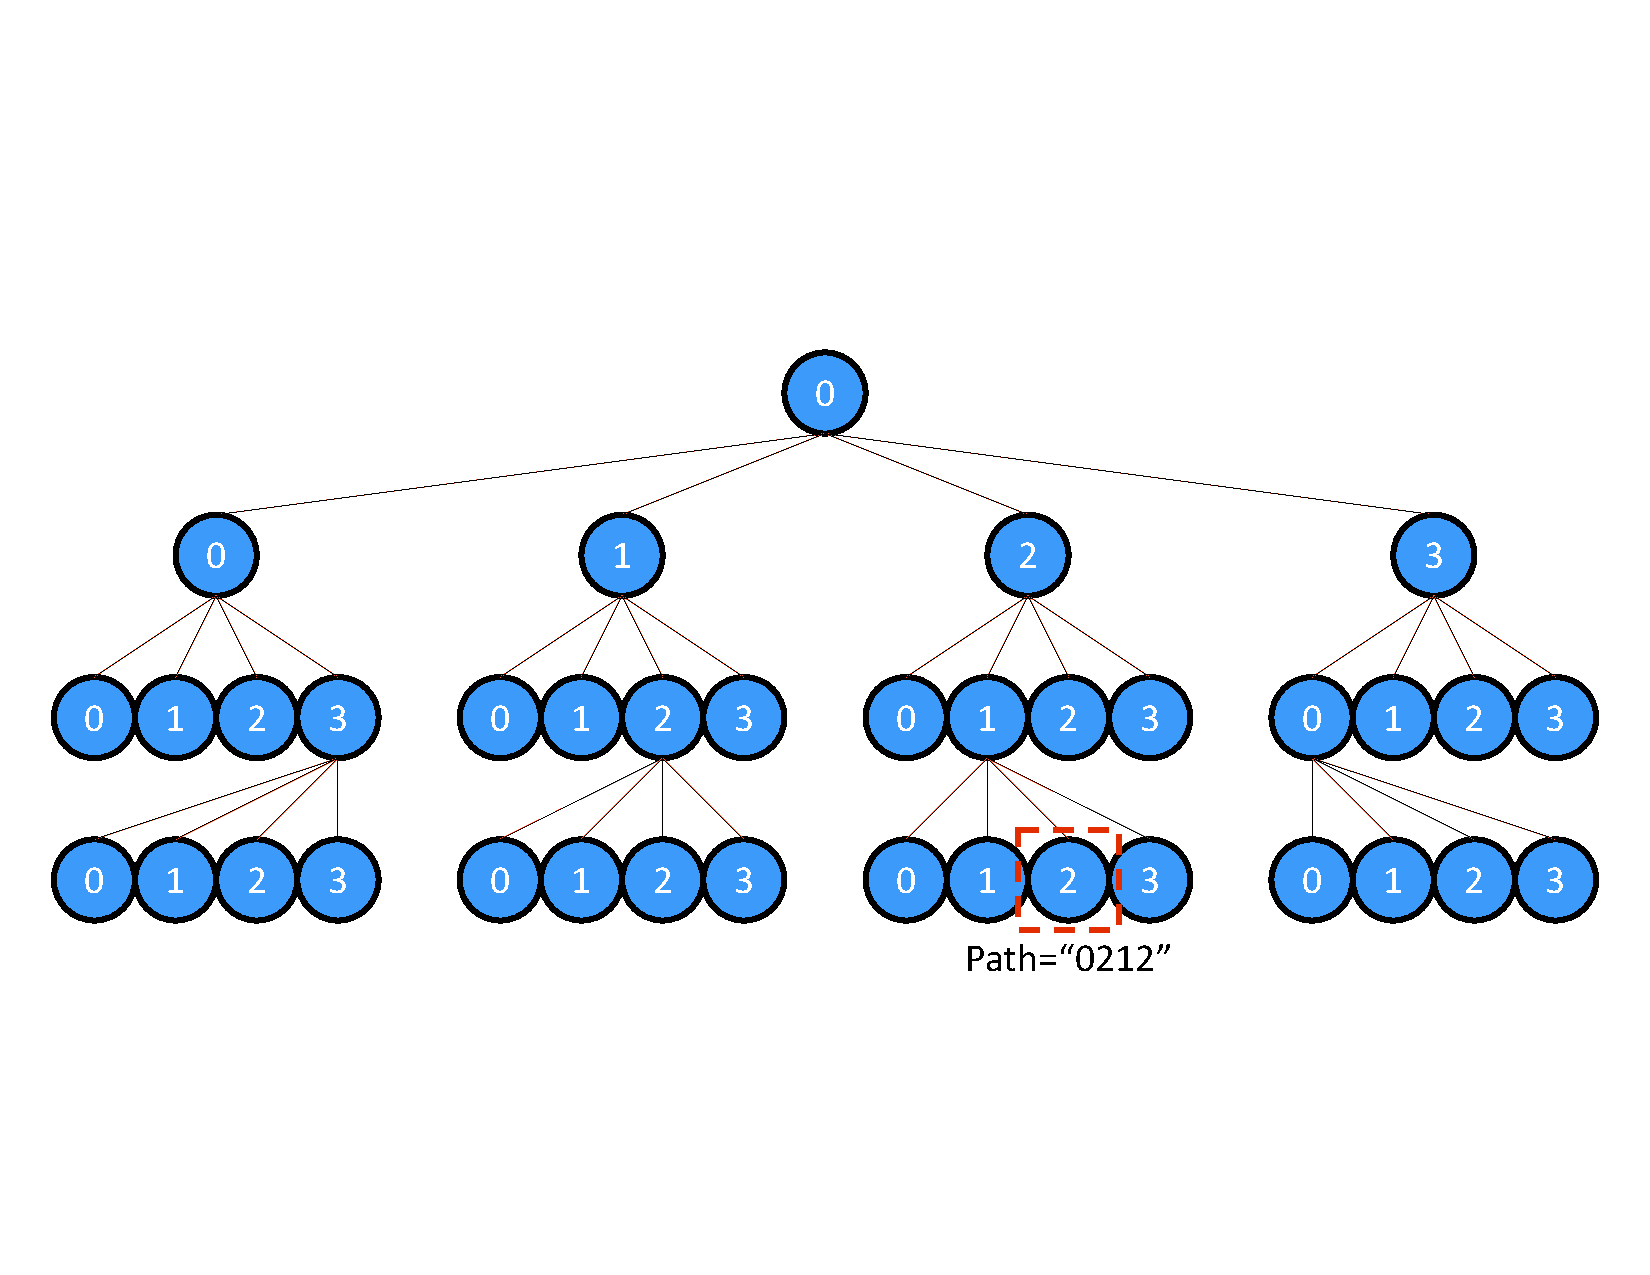
\includegraphics[width=\textwidth, clip=true, trim={0 140 0 150}]{figures/path-indexed-quadtree-serial.pdf}
            \caption{Path-indexed quadtree $\mathcal{Q}_P$}
            \label{subfig:path-indexed-quadtree-serial}
        \end{subfigure}
    \end{tabular}\\
    \caption{Leaf-indexed vs. path-indexed quadtrees. These represent the domain shown in \reffig{fig:adaptive-mesh-serial}. Note that the leaf-indexed quadtree only stores the leaf nodes (nodes without children), while the path-indexed quadtree stores all nodes (leaf and intermediate nodes).}
    \label{fig:quadtree-indexing-serial}
\end{figure}

% We focus on the constant coefficient elliptic problem
% \begin{equation}
%     \nabla^2 u(x,y) + \lambda u(x,y) = f(x,y), \quad \lambda \ge 0
%     \label{eq:elliptic_pde}
% \end{equation}
% with $(x,y) \in \Omega = [a, b] \times [c,d]$, subject to Dirichlet boundary conditions
% \begin{equation}
%     u(x,y) = g(x,y),\ \ (x,y) \in \Gamma = \partial \Omega.
% \end{equation}
% For this paper, we assume that $b-a=d-c$ so that we can describe our mesh using a single quadtree and square mesh cells.  In general though, this is not a limitation of meshes generated using the multi-block ``forest-of-octrees'' capabilities of \pforest.  The primary contributions of this paper are an HPS solver for the constant coefficient elliptic problem on an adaptively refined \pforest mesh. In future work, we will include fast linear algebra needed to reduce the complexity of the overall algorithm to $\mathcal O(N)$, a key contribution of the original HPS method developed by Gillman and Martinsson.